\section{The cross product}

\begin{outcome}

\begin{enumerate}

\item[A.] Compute the cross product and box product of vectors in $\mathbb{R}^3$.
\end{enumerate}
\end{outcome}

Recall that the dot product is one of two important products for vectors. The second type of product for vectors is called the cross product. It is important to note that the 
cross product is only defined in $\mathbb{R}^{3}$ and produces a vector. 
First we discuss the geometric meaning and then a description in terms of
coordinates is given, both of which are important. 
The geometric description is essential in order to understand the
applications to physics and geometry while the coordinate description is necessary to compute the cross product.
\index{right handed system}
\index{cross product}

Consider the following definition.

\begin{definition}{Right hand system of vectors}{righthand}
Three vectors, $\vect{u},\vect{v},\vect{w}$ form a right hand system if when you
extend the fingers of your right hand along the direction of vector $\vect{u}$ and
close them in the direction of $\vect{v}$, the thumb points roughly in the
direction of $\vect{w}$.
\end{definition}

For an example of a right handed system of vectors, see the following
picture.

\begin{center}
\begin{tikzpicture}
\draw[<->](-2,0,0)--(0,0,0)--(0,2,0);
\draw[->](0,0,0)--(0,0,3);
\node[above] at (-1,0,0){$\vect{u}$};
\node[right] at (0,0,1.5){$\vect{v}$};
\node[right] at (0,1,0){$\vect{w}$};
\end{tikzpicture}
\end{center}

In this picture the vector $\vect{w}$ points upwards from the plane
determined by the other two vectors. Point the fingers of your right hand along $\vect{u}$, and 
close them in the direction of $\vect{v}$. Notice that if you extend the thumb on your right hand,
it points in the direction of $\vect{w}$.

You should consider how a right hand
system would differ from a left hand system. Try using your left hand and
you will see that the vector $\vect{w}$ would need to point in the
opposite direction.

Notice that the special vectors, $\vect{i},\vect{j},\vect{k}$ will always form a right handed
system. If you extend the fingers of your right hand along $\vect{i}$ and 
close them in the direction $\vect{j}$, the thumb points
in the direction of $\vect{k}$.

\begin{center}
\begin{tikzpicture}
\draw[->, thick] (0,0,0)--(2,0,0);
\draw[->, thick] (0,0,0)--(0,2,0);
\draw[->, thick] (0,0,0)--(0,0,2);
\node[below right] at (2,0,0){$\vect{j}$};
\node[below left] at (0,0,2){$\vect{i}$};
\node[above right] at (0,2,0){$\vect{k}$};
\end{tikzpicture}
\end{center}

The following is the geometric description of the cross product. Recall that the dot product of 
two vectors results in a scalar. In contrast, the cross product results in a vector, as the product gives
a direction as well as magnitude.
\index{cross product!geometric description}

\begin{definition}{Geometric definition of cross product}{crossprodgeomet}
Let $\vect{u}$ and $\vect{v}$ be two vectors in $\mathbb{R}^{3}.$ 
Then the \textbf{cross product}, written $\vect{u}\times \vect{v}$, is defined by
\index{cross product} the following two rules.
\index{cross product!geometric description}

\begin{enumerate}
\item Its length is $\vectlength \vect{u}\times \vect{v}\vectlength =\vectlength \vect{u}\vectlength \vectlength
\vect{v}\vectlength \sin \theta $, \\
where $\theta $ is the included angle between $\vect{u}$ and $\vect{v}$.

\item It is perpendicular to both $\vect{u}$ and $\vect{v}$, that is $\left( \vect{u}\times \vect{v} \right) \dotprod \vect{u}=0,$ $\left( \vect{u}\times \vect{v} \right) \dotprod \vect{v}=0,$ \\
and  $\vect{u},\vect{v},\vect{u}\times \vect{v}$ form a right hand system.
\end{enumerate}
\end{definition}

The cross product of the special vectors $\vect{i}, \vect{j},
\vect{k}$ is as follows.  
\begin{equation*}
\begin{array}{cc}
\vect{i}\times \vect{j}=\vect{k} & \vect{j}\times \vect{i}=-\vect{k} \\
\vect{k}\times \vect{i}=\vect{j} & \vect{i}\times \vect{k}=-\vect{j} \\
\vect{j}\times \vect{k}=\vect{i} & \vect{k}\times \vect{j}=-\vect{i}
\end{array}
\end{equation*}
With this information, the following gives the coordinate description of the
cross product.
\index{cross product!coordinate description}

Recall that the vector $\vect{u}= \leftB 
\begin{array}{ccc}
u_1 & u_2 & u_3
\end{array}
\rightB^T$
can be written in terms of $\vect{i}, \vect{j}, \vect{k}$ as $\vect{u}=u_{1}\vect{i}+u_{2}\vect{j}+u_{3}\vect{k}$. 

The cross product satisfies the following properties.

\begin{proposition}{Properties of the Cross Product}{propertiescrossproduct}
Let $\vect{u}, \vect{v}, \vect{w}$ be vectors in $\mathbb{R}^3$, and $k$ a scalar. Then, the following properties 
of the cross product hold.
\begin{enumerate}
\item 
$\vect{u}\times \vect{v}= -\left( \vect{v}\times \vect{u}\right), 
\mbox{and} \; \vect{u}\times \vect{u}=\vect{0}$
\item 
$\left( k \vect{u}\right)\times \vect{v}= k \left( \vect{u}\times \vect{v}\right) 
=\vect{u}\times \left( k \vect{v}\right)$
\item
$\vect{u}\times \left( \vect{v}+\vect{w}\right) =\vect{u}\times \vect{v}+\vect{u}\times \vect{w}$
\item 
$\left( \vect{v}+\vect{w}\right) \times \vect{u}=\vect{v} \times \vect{u}+\vect{w}\times \vect{u}$
\end{enumerate}
\end{proposition}

\begin{proof}
Formula $1.$ follows immediately from the definition. The vectors 
$\vect{u}\times \vect{v}$ and $\vect{v}\times \vect{u}$ have the same magnitude, 
$\left\vert \vect{u}\right\vert \left\vert \vect{v}\right\vert \sin
\theta ,$ and an application of the right hand rule shows they have opposite
direction. 

Formula $2.$ is proven as follows. If $k $ is a
non-negative scalar, the direction of $\left( k \vect{u}\right)
\times \vect{v}$ is the same as the direction of $\vect{u}\times \vect{v},
k \left( \vect{u}\times \vect{v}\right) $ and $\vect{u}\times \left(
k \vect{v}\right) $. The magnitude is  $k$ times the
magnitude of $\vect{u}\times \vect{v}$ which is the same as the magnitude of 
$k \left( \vect{u}\times \vect{v}\right) $ and $\vect{u}\times \left(
k \vect{v}\right) .$ Using this yields equality in $2$. In
the case where $k <0,$ everything works the same way except the vectors
are all pointing in the opposite direction and you must multiply by 
$\left\vert k \right\vert $ when comparing their magnitudes. 

The distributive laws, $3.$ and $4.$, are much harder to establish. For now, it suffices to
 notice that if we know that $3.$ is true, $4.$ follows. Thus, assuming $3.$, and using $1.$,
\begin{align*}
\left( \vect{v}+\vect{w}\right) \times \vect{u}& =-\vect{u}\times \left(
\vect{v}+\vect{w}\right) \\
& =-\left( \vect{u}\times \vect{v}+\vect{u}\times \vect{w}\right) \\
& =\vect{v}\times \vect{u}+\vect{w}\times \vect{u}
\end{align*}
\end{proof}

\begin{proposition}{Coordinate Description of Cross Product}{crossprodcoord}
 Let $\vect{u}=u_{1}\vect{i}+u_{2}\vect{j}+u_{3}\vect{k}$
 and $\vect{v}=v_{1}\vect{i}+v_{2}\vect{j}+v_{3}\vect{k}$ be two
vectors. Then
\begin{equation}
\begin{array}{c}
\vect{u}\times \vect{v} 
 =\left( u_{2}v_{3}-u_{3}v_{2}\right) \vect{i}-\left(
u_{1}v_{3} - u_{3}v_{1}\right) \vect{j}+  \\
 +\left( u_{1}v_{2}-u_{2}v_{1}\right) \vect{k}  \label{crossprod1}
\end{array}
\end{equation}
\end{proposition}

Note that we will learn a quicker way to evaluate the cross product, further in this course when we learn about determinants.

Writing $\vect{u} \times \vect{v}$ in the usual way, it is given by 
\begin{equation*}
\vect{u} \times \vect{v}
=
\leftB
\begin{array}{r}
 u_{2}v_{3}-u_{3}v_{2} \\
-(u_{1}v_{3}-u_{3}v_{1}) \\
 u_{1}v_{2}-u_{2}v_{1}
\end{array}
\rightB
\end{equation*}

We now prove this proposition. 

\begin{proof} From the above table and the properties of the cross
product listed,
\begin{eqnarray*}
\vect{u} \times \vect{v} &=& \left( u_{1}\vect{i}+u_{2}\vect{j}+u_{3}\vect{k}\right) \times \left(
v_{1}\vect{i}+v_{2}\vect{j}+v_{3}\vect{k}\right) \\
&=& u_{1}v_{2}\vect{i}\times \vect{j}+u_{1}v_{3}\vect{i}\times \vect{k}+u_{2}v_{1}\vect{j}\times \vect{i}+
u_{2}v_{3}\vect{j}\times \vect{k}+
+u_{3}v_{1}\vect{k}\times \vect{i}+u_{3}v_{2}\vect{k}\times \vect{j} \\
&=&u_{1}v_{2}\vect{k}-u_{1}v_{3}\vect{j}-u_{2}v_{1}\vect{k}+u_{2}v_{3}
\vect{i}+u_{3}v_{1}\vect{j}-u_{3}v_{2}\vect{i} \\
&=&\left( u_{2}v_{3}-u_{3}v_{2}\right) \vect{i}+\left(
u_{3}v_{1}-u_{1}v_{3}\right) \vect{j}+\left( u_{1}v_{2}-u_{2}v_{1}\right)
\vect{k}  
\end{eqnarray*}
\begin{equation}
\label{crossprod2}
\end{equation}
\end{proof}

\begin{comment}
There is another version of \ref{crossprod1} which may be easier to remember.
We can express the cross product as the determinant of a matrix, as follows. 
\begin{equation}
\vect{u}\times \vect{v} = \left\vert
\begin{array}{ccc}
\vect{i} & \vect{j} & \vect{k} \\
u_{1} & u_{2} & u_{3} \\
v_{1} & v_{2} & v_{3}
\end{array}
\right\vert  \label{crossprod3}
\end{equation}
Expanding the determinant along the top row yields
\begin{equation*}
\vect{i}\left( -1\right) ^{1+1}\left\vert
\begin{array}{cc}
u_{2} & u_{3} \\
v_{2} & v_{3}
\end{array}
\right\vert +\vect{j}\left( -1\right) ^{2+1}\left\vert
\begin{array}{cc}
u_{1} & u_{3} \\
v_{1} & v_{3}
\end{array}
\right\vert +\vect{k}\left( -1\right) ^{3+1}\left\vert
\begin{array}{cc}
u_{1} & u_{2} \\
v_{1} & v_{2}
\end{array}
\right\vert
\end{equation*}
\begin{equation*}
=\vect{i}\left\vert
\begin{array}{cc}
u_{2} & u_{3} \\
v_{2} & v_{3}
\end{array}
\right\vert -\vect{j}\left\vert
\begin{array}{cc}
u_{1} & u_{3} \\
v_{1} & v_{3}
\end{array}
\right\vert +\vect{k}\left\vert
\begin{array}{cc}
u_{1} & u_{2} \\
v_{1} & v_{2}
\end{array}
\right\vert
\end{equation*}
Expanding these determinants leads to 
\begin{equation*}
\left( u_{2}v_{3}-u_{3}v_{2}\right) \vect{i}-\left(
u_{1}v_{3}-u_{3}v_{1}\right) \vect{j}+\left( u_{1}v_{2}-u_{2}v_{1}\right)
\vect{k}  
%\label{crossprod4}
\end{equation*}
which is the same as \ref{crossprod2}.
\end{comment}

We will now look at an example of how to compute a cross product.

\begin{example}{Find a cross product}{findcrossproduct}
Find $\vect{u} \times \vect{v}$ for the following vectors
\begin{equation*}
\vect{u}
=
\leftB
\begin{array}{r}
1 \\
-1 \\
2
\end{array}
\rightB,
\vect{v}
=
\leftB
\begin{array}{r}
3 \\
-2 \\
1
\end{array}
\rightB
\end{equation*}
\end{example}

\begin{solution}
Note that we can write $\vect{u}, \vect{v}$ in terms of the special vectors $\vect{i},
\vect{j}, \vect{k}$ as 
\begin{equation*}
\begin{array}{c}
\vect{u}
=
\vect{i}-\vect{j}+2\vect{k} \\
\vect{v}
=
 3\vect{i}-2\vect{j}+\vect{k}
\end{array}
\end{equation*}

We will use the equation given by \ref{crossprod2} to compute the cross product. 
\begin{equation*}
\vect{u} \times \vect{v}
=((-1)(1)-(2)(-2)) \vect{i}- ((1)(1)-(1)(3)) \vect{j}+((1)(-2)-(-1)(3)) \vect{k}=3\vect{i}+5\vect{j}+\vect{k}
\end{equation*}

We can write this result in the usual way, as
\begin{equation*}
\vect{u} \times \vect{v}
=
\leftB
\begin{array}{r}
3 \\
5 \\
1
\end{array}
\rightB
\end{equation*}

\end{solution}

An important geometrical application of the cross product is as follows. The size of the cross product, $\vectlength \vect{u}\times \vect{v}\vectlength $, is the area of the
parallelogram determined by $\vect{u}$ and $\vect{v}$, as shown in the following picture. 
\index{cross product!area of parallelogram}

\begin{center}
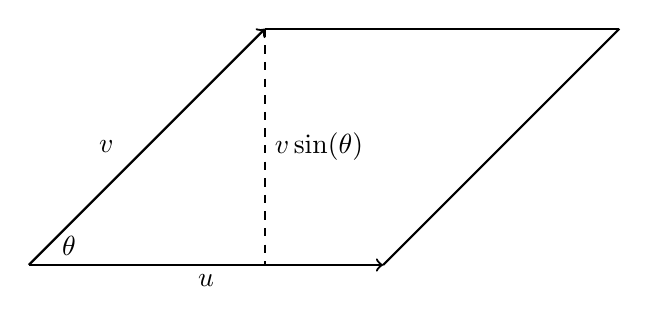
\begin{tikzpicture}[scale=1.5]
\draw[->,thick](0,0)--(2,2);
\draw[->,thick](0,0)--(3,0);
\draw[thick](2,2)--(5,2);
\draw[thick](3,0)--(5,2);
\draw[dashed](2,2)--(2,0);
\node[below] at (1.5,0){$\vect{u}$};
\node[left] at (0.8,1){$\vect{v}$};
\node[above right] at (0.2,0){$\theta$};
\node[right] at (2,1){$\vectlength \vect{v} \vectlength \sin(\theta)$};
\end{tikzpicture}
\end{center}

We use this concept in the following example.

\begin{example}{Area of a parallelogram}{areaparallelogram}
Find the area of the
 parallelogram determined by the vectors $\vect{u}$
and $\vect{v}$ given by 
\begin{equation*}
\vect{u}
=
\leftB
\begin{array}{r}
1 \\
-1 \\
2
\end{array}
\rightB, 
\vect{v}
=
\leftB
\begin{array}{r}
3 \\
-2 \\
1
\end{array}
\rightB
\end{equation*}
\end{example}

\begin{solution}
Notice that these vectors are the same as the ones given in Example \ref{exa:findcrossproduct}.
Recall from the geometric description of the cross
product, that the area of the parallelogram is simply the magnitude of $\vect{u} \times \vect{v}$. 
From Example \ref{exa:findcrossproduct}, $\vect{u} \times \vect{v} = 3\vect{i}+5\vect{j}+\vect{k}$.
We can also write this as
\begin{equation*}
\vect{u} \times \vect{v}
=
\leftB
\begin{array}{r}
3 \\
5 \\
1
\end{array}
\rightB
\end{equation*}

Thus the area of the parallelogram is 
\begin{equation*}
\vectlength \vect{u} \times \vect{v} \vectlength = 
\sqrt{(3)(3) + (5)(5) + (1)(1)} = 
\sqrt{9+25+1}=\sqrt{35}
\end{equation*}
\end{solution}

We can also use this concept to find the area of a triangle. Consider the following
example.

\begin{example}{Area of triangle}{areatriangle}
Find the area of the triangle determined by the points $\left(1, 2, 3 \right) ,
\left( 0,2,5\right),
\left( 5,1, 2 \right) $ 
\end{example}

\begin{solution}
This triangle is obtained by connecting the three points with lines. Picking
$\left( 1,2,3\right) $ as a starting point, there are two displacement
vectors, $\leftB 
\begin{array}{rrr}
-1 & 0 & 2
\end{array}
\rightB^T $ and $\leftB 
\begin{array}{rrr}
4 & -1 & -1
\end{array}
\rightB^T $. Notice that if we add either of these vectors to the position vector of the 
starting point, the result is the position vectors of the other two
points. Now, the area of the triangle is half the area of the parallelogram
determined by $\leftB 
\begin{array}{rrr}
-1 & 0 & 2
\end{array}
\rightB^T $ and $\leftB 
\begin{array}{rrr}
4 & -1 & -1
\end{array}
\rightB^T.$ 
The required cross product is given by
\begin{equation*}
\leftB 
\begin{array}{r}
-1 \\
0 \\
2
\end{array}
\rightB \times \leftB 
\begin{array}{r}
4 \\
-1 \\
-1
\end{array}
\rightB = \leftB
\begin{array}{rrr}
2 \\ 7 \\ 1
\end{array}
\rightB 
\end{equation*}
  Taking the size of this vector gives the area of the parallelogram,
given by 
\begin{equation*}
\sqrt{(2)(2) + (7)(7) + (1)(1)}
=
\sqrt{4+49+1}
= \sqrt{54}
\end{equation*}
Hence the area of the triangle is $\frac{1}{2}\sqrt{54}= \frac{3}{2}\sqrt{6}.$
\end{solution}

In general, if you have three points in $\mathbb{R}^{3}, P,Q,R$, the area of the triangle is given by
\begin{equation*}
\frac{1}{2}\vectlength  \longvect{PQ} \times  \longvect{PR}  \vectlength 
\end{equation*}

Recall that $\longvect{PQ}$ is the vector running from point $P$ to point $Q$. 

\begin{center}
\begin{tikzpicture}
\draw[->](0,0)--(2,2);
\draw[->](0,0)--(4,0);
\draw(2,2)--(4,0);
\node[left] at (0,0){$P$};
\node[above] at (2,2){$Q$};
\node[right] at (4,0){$R$};
\end{tikzpicture}
\end{center}

In the next section, we explore another application of the cross product.